% !TeX root = Project.tex
\section{Approximating area --- Riemann Style}

This is the code I wrote to draw the sequence of approximations shown in Figure \ref{fig:areaapprox}. It can be used to visualise the approximation of the Integral of any function in a \dref{def:riemann}[\emph{`Riemann style'}] --- given that you already have a way to write it as a Python function with the form:

\begin{minted}{python}
# f(x) -----> number.
\end{minted}

It can be modified easily to produce quite a few of approximations - here we just set n to 6.

\begin{minted}{python}
import matplotlib.pyplot as plt
import numpy as np 

n = 6
\end{minted}

First, we want to set the limits of integration, $[a, b]$, and use this to calculate a total width.

\begin{minted}{python}
xmax = 6
xmin = 0
totalwidth = xmax - xmin
\end{minted}

Then we use this, and our n, to split up the axis into $5 \times 2^{n-1}$ equal sized sections. We will divide the lengths of each bar by 2 every step of the approximation, so this ensures that our coarsest approximation has 5 bars. 
\begin{minted}{python}
# 160 points equally spaced points (plus zero) in the domain
num = (5 * 2**(n-1)) + 1
x = np.linspace(xmin, xmax, num=num, endpoint=True)
\end{minted}

Define the function of interest, $f$.
Calculate $y$ values to plot a graph. 

\begin{minted}{python}
# Make a list of 'n' colours
colour1 = '#95d0fc' #light blue
colour2 = '#75bbfd' #sky blue
colour3 = '#00ffff' #cyan
colour4 = '#13eac9' #aqua
colour5 = '#929591' #grey
colour6 = '#06c2ac' #turquoise
colour = [colour1, colour2, colour3, colour4, colour6, colour5]

f = np.sin
y = f(x)

# To draw graph
xs = np.linspace(xmin, xmax, 100)
ys = f(xs)

fig, axesr = plt.subplots(nrows=int(n/2), ncols=2, dpi=300, figsize=(5, n*3/4))
fig.subplots_adjust(hspace = 0.075)
axes = [ax for axes in axesr for ax in axes]

fig.subplots_adjust(wspace=0.05, hspace=0.075)

for ax in axes:
    ax.plot(xs, ys, 'g-', linewidth=0.5) 
    ax.tick_params(top=False, 
                   bottom=False, 
                   left=False, 
                   right=False, 
                   labelleft=False, 
                   labelbottom=False, 
                   labelright=False,
                   labeltop=False)
    for axis in ['top','bottom','left','right']:
      ax.spines[axis].set_linewidth(0.4)

    ax.set_xlim(xmin, xmax)    
\end{minted}
    
A quick explanation of this next step is that it's setting up the \dref{def:stfun}[\emph{`representations'}] of the
\dref{def:stfun}[\emph{Step Functions}] used to approximate the function of interest. Those sequences are defined by $$x_{n,m} = x_{n,m-1} + \frac{totalwidth}{5 \times 2^{n-1}}$$

In this example, I am bounding the function from below, but by changing 'min' to 'max', you can bound it from above.

\begin{minted}{python}
reps = [x[:-1:2**n] for n in range(n)]
bars = [(x, []) for x in reps]
for interval_steps, bar in zip(reps, bars):
    for i in range(len(interval_steps)):
        xright = xmax if i == len(interval_steps) - 1 else interval_steps[i+1]
        xleft = interval_steps[i]
        interval = np.linspace(xleft, xright, 1000)
        interval_mapped = [f(x) for x in interval]
        interval_min = min(interval_mapped) ## Can change 'min' to 'max'
        bar[1].append(interval_min)         ## to bound from above
\end{minted}
      
Now we can plot the bars at the right heights, using the colours we picked earlier.  Also, what I mean by \emph{`bounding from below'} is that we are finding the \dref{def:hseq}[\emph{height sequence}] where every height is the greatest lower bound (infinium) of the values the function takes in the corresponding step. But that's a bit of a mouthful.

\begin{minted}{python}
i = n
for ax in reversed(axes):
    i -= 1
    div = 5 * 2**i
    ax.bar(*bars[n-i-1], 
        align='edge', width=(totalwidth/div), 
        fc=colour[i], ec=colour[i], alpha=0.95)

fig.savefig('RiemannExample.png')
\end{minted}

\begin{figure}[H]
\centering
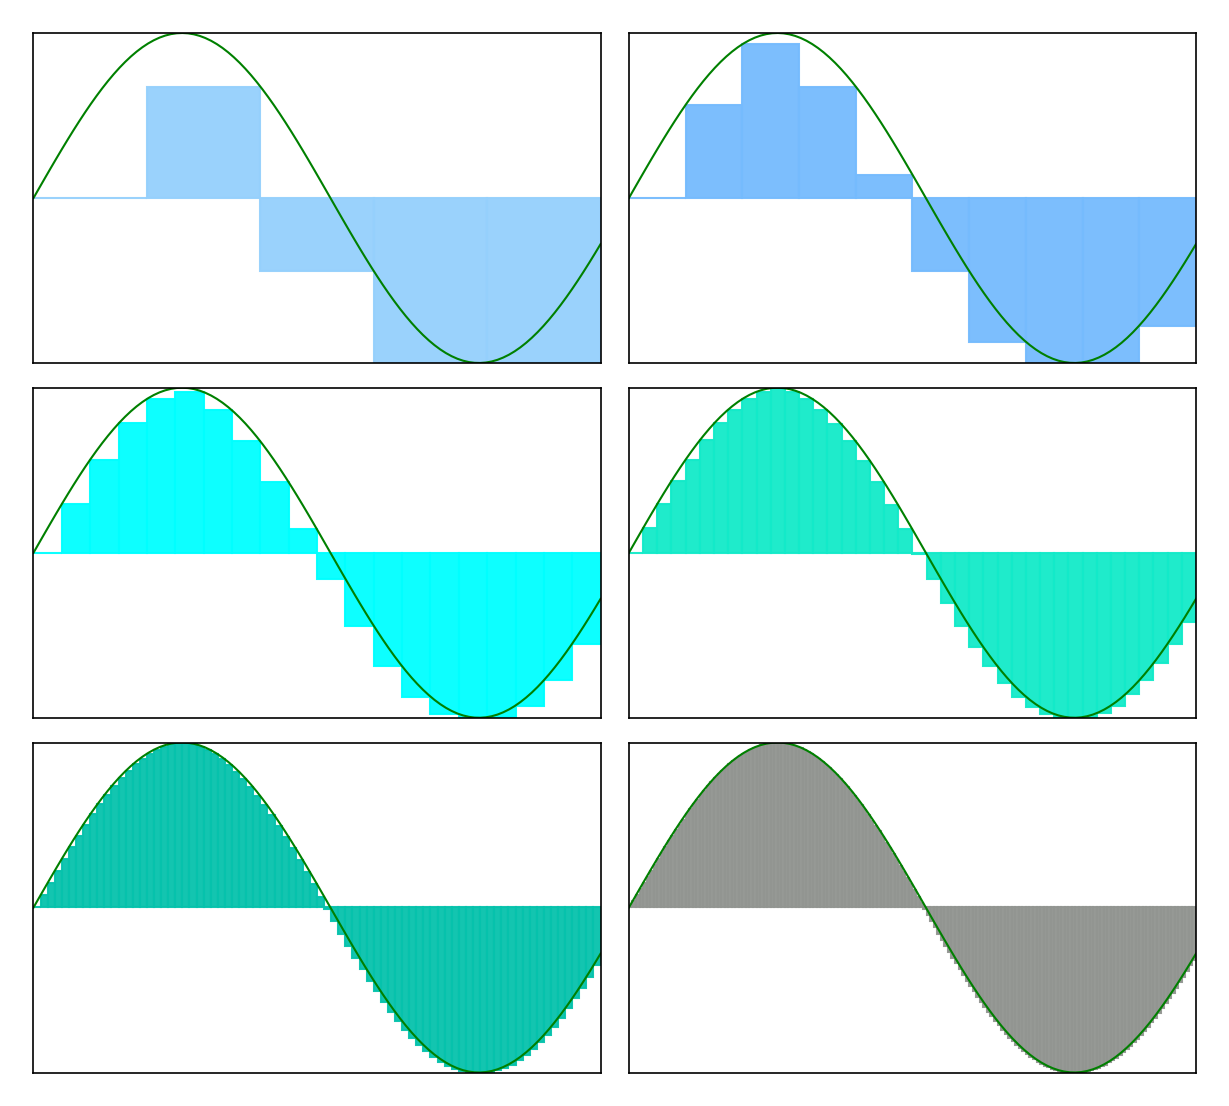
\includegraphics{Code/RiemannExample.png}
\caption{RiemannExample.png}
\end{figure}